\documentclass[a4paper,10pt]{article}
\usepackage[utf8]{inputenc}
\usepackage{graphicx}
\usepackage{lingsty,ipashortcuts,gb4n}
\usepackage{tipa}
\usepackage{textcomp}
\usepackage{multirow}
\usepackage{array}
\usepackage{rotating}
\usepackage{anysize}
\usepackage{graphicx}
\marginsize{2.5cm}{2.5cm}{2.5cm}{2.5cm}

\usepackage[authoryear]{natbib}

\newcommand{\teitag}[1]{\texttt{$<$#1$>$}}

%opening
\title{Archiving Grammatical Descriptions}
\author{Sebastian Nordhoff \& Harald Hammarstr\"om}
% \institute{Max Planck Institute for Evolutionary Anthropology}
\begin{document}

\maketitle

\begin{abstract}
  We argue that grammatical descriptions should be archived not in a monolithic but in a granular way, making use of the framework of the Text Encoding Initiative. We show how tags of the extant framework and additions crafted for descriptive linguistics can be applied to linguistic text. Granular annotation with Uniform Resource Identifiers for all elements will allow grammatical descriptions (and their parts!) to become part of the Semantic Web. We add to existing formalizations of low-level elements by providing a schema for the higher order organization of grammatical descriptions and discuss how legacy descriptions can be parsed and annotated in a scalable manner.
\end{abstract}

keywords: archiving, grammatical description, schema, linked data, named entity recognition, latent semantic analysis

\section{Archives}
There are several aspects to archiving, whose importance varies according to the discipline. The  origin of archiving is archiving artifacts, i.e. physical objects (a vase, an axe, a book). In  recent years, there has been a movement towards digital archiving, where one archives a \em representation \em of an artifact (a 3D-model of a vase or an axe, a scan of a book), i.e. a digital surrogate of the artifact. The last aspect finally is archiving content, which only works for artifacts containing text. Here we are not concerned with the physical form (quart, folio, parchment, papyri), but rather with the string of characters making up the document.  

When archiving a grammatical description, we can illustrate the three aspects just mentioned as follows: you can archive the printed book (the artifact) and take care of optimal conditions regarding humidity, temperature, exposure to sunlight etc. Or you could archive a *tiff-scan of the book where every page is represented in excellent resolution and color depth. This would be a representation of the artifact. In this case, you lose non-visual information, like touch or smell of the book. Finally, you could archive the string of characters which make up the content of the book. Here you lose visual information as well (colour, page layout, exact font used, miniatures etc.), although some of it can be recorded as meta-information.

In the context of grammatical description, the last aspect (archiving content) is clearly the most important. While there are some masterpieces of editorship in the grammatical literature, what is produced in language documentation normally excels by content rather than layout, typeset or paper choice. What is to be preserved for future generations is the content, not necessarily the physical arrangement of glyphs on a support. This is even more the case for documents "born-digital" where the physical support does not exist until the user prints the document. References to the  physical shape of the document (page breaks, line breaks) can also be stored, but this is not central here.

Concerning archiving texts, we can make two further distinctions: either archive the whole text as a monolithic block without internal structure, a very long array of characters so to speak, or use a more granular approach and record the elements which constitute the text (headings, sections, footnotes, cross-references, etc). This more granular approach allows for easier search for particular items in the text, allows for easier updates if necessary, and allows for easier  integration in the Semantic Web. In the remainder of this paper, I will advocate such a granular approach to archiving grammatical descriptions using the framework of the Text Encoding Initiative \citep[TEI,][]{TEIGuidelines}.

With regard to archives, we can distinguish two more axes: orientation and perfectivity. The first axis, orientation, refers to the focus of the archive being inward or outward: Is it important to get stuff into the archive (store), or is it important to get stuff out of the archive to the interested user (serve)? A good archive will necessarily try to serve both functions as well as possible, but scarcity of resources means that often a choice has to be made. The second axis, which I term perfectivity, in analogy to the distinction in linguistic aspect, refers to the state of completeness an archive requires. A `perfective' archive only accepts finished documents. It is not possible to modify archived documents. The archive is read-only, so to speak.  A non-perfective archive will store whatever there is, without requiring completedness.It is always possible to modify parts of the archived content. A version history can of course be kept to assure that the evolution of the content can be traced. I will assume an outward-oriented, non-perfective archive as the right paradigm for grammatical descriptions.

\citet{Good2004} conceives of a grammatical description as a meta-database of nested `annotations'. The grammatical description is seen as a collection of short chunks, which are largely independent of each other, but with explicit relations to each other. \citet{Nordhoff2008jldc} argues that grammatical descriptions are best seen as non-linear texts (i.e. hypertexts) where every individual reader will follow their own path of exploration (skip phonology, start with syntax, jump back to morphology as required, use table of contents and index extensively).

The use of rather atomic linguistic facts as the basis of the creation of linguistic knowledge has been argued for by \citet{Cysouw2009micropub}, who advocates the use of `micro-publications', very short statements about one linguistic fact of one particular language. To pull the ideas of these three authors together: A grammatical description is a non-linear meta-database of micropublications.

A granular approach jibes well with this model, as items can be added or modified on a local basis, whereas in the monolithic approach, every local modification would also be a global modification. The granular approach also allows easier serving of particular chunks, because of easier retrieval. Finally, a granular approach will allow to uniquely identify chunks and refer to them in Semantic Web frameworks such as RDF\footnote{http://www.w3.org/RDF/} or OWL.\footnote{http://www.w3.org/TR/owl-features/}


\section{Granular text}
Let us illustrate the meaning of granular text with an example

\begin{verbatim}
 <div id="ch3" type="chapter" n="3" >
  <head>Morphology</head>
  <div id="ch3s1" type="section" n="1">
   <head>Nominal morphology</head>
   <p>
    In contrast to <ref target="#verbalmorphology"> verbal morphology
    </ref> Nominal morphology is very important in <languagename iso6393="qqq">
    Ugubugu</languagename>. This can be seen from example <ptr target="#ch3s1ex1" />.
    Especially the <technicalterm    ontology="GOLD" value="case marker">case marker
    </technicalterm> <phraseglosspair><phrase lg="qqq">ka</phrase><gloss type="Leipzig">
    ACC</gloss></phraseglosspair> is important here.
   </p>
   <lgex id="ch3s1ex1" number="1">
    <sourceline> ... </sourceline>
    <interlinear> ... </interlinear>
    <translationline> </translation>
   </lgex>
  </div>
 </div>
\end{verbatim}

We can observe a number of points from the example above:

\begin{enumerate}
 \item Important elements in the texts like headings, examples, or cross-references are explicitly labelled
 \item There are unique references to paragraphs and examples.
 \item Some terms are enclosed in semantic markup. This includes technical terms and object language terms.
 \item The semantic markup includes references to definitions of the terms used, in the case the GOLD ontology\footnote{http://linguistics-ontology.org/} and the Leipzig Glossing Rules.\footnote{http://www.eva.mpg.de/lingua/resources/glossing-rules.php}
\end{enumerate}

This markup combined with unique references allows to integrate such a chunk into the semantic web. For instance, one could retrieve all sections of grammatical descriptions in the archive which make reference to the concept of "case marker" as defined in GOLD, even if the actual terms employed differ.
 
\section{Linked Data}
We will briefly illustrate the usefulness of such a granular resource within the Linked Data paradigm \citep{HeathEtAl2011}, without going into too much detail. The five steps for Linked Data are \citep{BernersLee2006}.

\begin{itemize}
 \item[*]       make your stuff available on the Web (whatever format) under an open license
 \item[**]	make it available as structured data (e.g., Excel instead of image scan of a table)
 \item[***]	use non-proprietary formats (e.g., CSV instead of Excel)
 \item[****]	use URIs to identify things, so that people can point at your stuff
 \item[*****]	link your data to other data to provide context
\end{itemize}
 
A granular approach to grammatical descriptions has the advantage that we can use the granular entities as parts of semantic statements. We can say "This section covers a topic which is also found in GOLD" or "This section is a close, but not perfect, match of what is found in GOLD".

Three things are important in order to arrive at such a generalization: The arguments of the relation must be identifiable, they must have Uniform Resource Identifiers (URIs); the relation must be defined; and the formalism to link the relation and the arguments must be established.

URIs can, for the purpose of this paper, be equated with web addresses of a certain format. Relations are defined in a number of vocabularies, of which RDFS\footnote{http://www.w3.org/TR/rdf-schema/}, OWL, Dublin Core\footnote{http://dublincore.org/}, SKOS\footnote{http://www.w3.org/2004/02/skos/}, GOLD and lexvo\footnote{http://www.lexvo.org/} are the most important ones for descriptive linguistics. The formalism to link those together, finally, is RDF\footnote{http://www.w3.org/RDF/}, here represented in a variant called N3\footnote{http://www.w3.org/DesignIssues/Notation3.html}. There is no space here to discuss details, but an example will show the general approach:
 
\ea <grammararchive:123/chapter/4/section/5>  <rdfs:seeAlso> <gold:Infix> .  \z

RDF predications are written in SVO (i.e. predicate-medial) notation. In this case, Chapter 4, Section 5 of the book with the ID 123 is the subject, \texttt{gold:Infix} in GOLD is the object, and the two are linked by the `verb', the predicate \texttt{rdfs:seeAlso}. Crucially, all of the three items are \em dereferenceable\em, which means that a definition of what they mean can be looked up on the Internet.\footnote{The actual Internet addresses have been abbreviated here, one would look up
http://www.grammararchive.org/grammar/123/chapter/4/section/5\\
http://www.w3.org/2000/01/rdf-schema\#seeAlso\\
http://linguistics-ontology.org/gold/2010/Infix.
}

The take-home message here is that only a granular approach with transparent URIs allows archived grammatical descriptions to be incorporated into the Semantic Web.


\section{Textual elements in linguistics}
In order to create a schema for grammatical descriptions, one needs to take stock of the elements which are found in this type of work. There are some elements which are share with other types of texts, such as paragraphs, headings, or cross-references. For those, the vocabulary provided by the TEI can be used. In linguistic texts, there are also a number of elements not listed in TEI. These will be discussed below.

\subsection{Named entities}
Named entities refer to concepts which have a definition of the particular text under discussion. Examples include countries, cities, persons, but also languages, books and linguistic concepts. Named entities are enclosed in the relevant semantic markup. An example is provided below.

\begin{verbatim}
<language iso639-2="cpp">Diu Indo-Portuguese</> is spoken in the
 <city geonamesID="1272502">city of Diu</city> in the <country
 ISO-3166-1="IN">Indian></country> <province ISO-3166-2="IN-DD">
 territory  of Daman and Diu</province>. <person gnd="118611046">
 Hugo Schuchardt</person> and <person gnd="115161023"> Sebastião
 Dalgado</person> provided the first description of this dialect;
 the latest work is Cardoso's <book ISBN="978-90-78328-87-2">A
 grammar of Indo-Portuguese</book>. 
\end{verbatim}
 
The extraction of named entities from a given text (Named Entity Recognition) is an important subfield of computational text linguistics \citep[e.g.][]{Borthwick1999}.

Linguistic concepts can be also be treated as named entities if they are defined outside of the text under discussion. Place where such concepts are defined include GOLD or lexvo for instance. An example is given below.

\begin{verbatim}
 <languagename iso639-3="tgl"> Tagalog </languagename> has
 <technicalterm GOLD="Infix">infixes</technicalterm>.
\end{verbatim}


\subsection{Object language}
In linguistic texts, frequent reference is made to languages which are not the metalanguage of the text. These are commonly typeset in italics. A semantic representation would be as follows.

\begin{verbatim}
 Italian <objectlanguage iso639-3="ita">cinque</objectlanguage>
 corresponds to Spanish <objectlanguage iso639-3="spa">cinco
 </objectlanguage>.
\end{verbatim}

The attribute \texttt{iso639-3} refers to the ISO 639-3 code\footnote{http://www.sil.org/iso639-3/} of the language.

\subsection{Phrase-gloss pairs}
Grammatical descriptions very often provide translations of object language terms directly after them.

\begin{verbatim}
 Spanish <phraseglosspair><phrase iso639-3="spa"> dolor </phrase><gloss
 iso639-3="eng">pain</gloss><phraseglosspair> preserves Latin intervocalic
 l, while Portuguese    <phraseglosspair><phrase iso639-3="por"> dor 
 </phrase><gloss iso639-3="eng">pain</gloss><phraseglosspair> does not.
\end{verbatim}


\subsection{Exemplars}
The most salient textual element found in grammars is the example, of which the traditional three-line interlinear glossed text is the best known. It is not the case, however, that this traditional three-liner provides a sufficient model of examples used in linguistic texts. In Marian Klamer's \em A Grammar of Teiwa \em \citep{g:Klamer:Teiwa}, only 40\% of the examples conform to a rigid specification of a three line text with the same number of tokens in the first and second lines. The other 60\% deviate from this model in one way or another (subexamples, missing lines, extra lines, missing quotation marks around translations etc.).

For these reasons, we have to specify an \em example container\em, which provides the numbering and a paragraph where the actual linguistic content can be found. This content can be of varying nature. We have found the following to be recurring types, but there might be more:

\begin{itemize}
 \item three-liners with interlinear morpheme translation
 \item two liners with lexeme and gloss
 \item two liners with tones and lexemes
 \item two-liners for minimal pairs
 \item one liners with lexeme$<$etymology
 \item ungrammatical one-liners
 \item ungrammatical one-liners with IMT but no translation
 \item three liners with lexeme, phonetic transcription, gloss, no translation
 \item four-liners with orthographic text, phonetic text, IMT, gloss
 \item four-liners with orthographic text, morphemes, IMT, gloss
 \item four-liners with intonation, text, IMT, gloss
 \item ...
\end{itemize}

We will not provide a full specification for all the subtypes of examples listed here. Schemas for some of those types can be found in \citet{BowEtAl2003}.

A linguistic example can either occur within a paragraph or between paragraphs. In the latter case, it has to be included in an otherwise empty paragraph

\begin{verbatim}
<p>
 English shows subject-verb agreement as 
 <examplecontainer n="1">
  <example type="oneliner"> 
   <exline type="objectlanguage" iso639-3="eng">The dog bark*(s)</exline>
  </example>
 </examplecontainer>
shows. This is also found in French, Spanish, and German (see below).
</p>

<p>
 <examplecontainer n="2">
  <example type="threeliner>
   <exline type="objectlanguage" iso639-3="fra">Tu regarde-*(s)</exline>
   <exline type="IMT">2s watch-2s</exline>
   <exline> 'You are watching.'</exline>
  </example>
 </examplecontainer>
</p>

<p>
 <examplecontainer n="3">
  <example type="threeliner>
   <exline type="objectlanguage" iso639-3="spa">(Tu) mira*(s)</exline>
    ...
  </example>
 </examplecontainer>
</p>

<p>
 <examplecontainer n="4">
  <example type="threeliner>
   <exline type="objectlanguage" iso639-3="fra">Du sieh-*(st)</exline>
   ...
  </example>
 </examplecontainer>
</p>
 
\end{verbatim}

Linguistic examples are techincally $n\times m$ tables. These can be serialized either horizontally (cells are elements of rows) or vertically (cells are elements of columns). Both solutions have their advantages, and they can be transformed into each other, so that this is a matter of personal taste. Linguistic example tables, like any other table, take up a lot of space when written in XML; therefore they are not formalized here. 

\subsection{Paradigms}
Another textual element frequently found in linguistic works is the paradigm. This is a special kind of table. Its formalization is quite complex, so that the reader is referred to \citet{PentonEtAl2004} here.

\subsection{References}
Linguistic texts contains many references. These are of different types. There are references to items in the text, like examples or other chapters. For these, the existing TEI-elements \texttt{$<$ref$>$} and \texttt{$<ptr>$} (pointer) can be used. References to items outside the text can be divided into references to the origin of the material (corpus, dictionary), and references to the literature. References to the literature can be handled with the existing TEI elements \teitag{biblstruct} and \teitag{listbibl}. References to a corpus or a dictionary are encoded as attributes of the element they refer to.

\begin{verbatim}
 The <language iso639-3="sci">Sri Lanka Malay</language> word 
<phraseglosspair><phrase iso639-3="sci" src="Nordhoff2009">
thaanàm</phrase><gloss iso639-3="eng">to plant</gloss>
</phraseglosspair> is also found in the <langauge linguasphere="">
Jakarta dialect of Indonesian<language> <bibitem src="Adelaar1985"
 isbn="978-0858834088"/>
 This is discussed in more detail in section <ptr target="Jakartan Influence" />
\end{verbatim}

\subsection{Tables and Figures}
Tables and figures can be handled according to the general TEI-guidelines, which provide the elements \teitag{table} and \teitag{figure}. A special kind of table found in linguistic descriptions is the phoneme chart. Due to the lengthy nature of table descriptions in XML, this will not be illustrated here.
 
\section{Markup philosophies}
There are two types of markup which are commonly used when describing the structure of a text. The examples above have all been in so-called \em inline \em markup. This means that the metainformation abouth the text, tags in this case, is found interspersed within the actual content. The alternative is standoff markup. In this case, the text is left untouched and the markup is written to another file. The stretch of text to which a particular markup refers is indicated by character counts, the offset, for instance (8,23) to refer to the stretch of characters from the 8th character to the 23rd character.

Standoff markup has the advantage that one does not need write access to the file one describes. The archive could just provide a read-only copy, and the annotation can be store at another location. Multiple, overlapping, or even conflicting annotations can be provided. The drawback of standoff annotations is that they are more difficult to read, and their vulnerability to changes in character count. Suppose you have the Dutch word \em Frankrÿk \em in a text, which consists of 8 letters. Later, you decide to use the more standard spelling \em Frankrijk\em. This changes the offset of all following characters by one, invalidating all standoff markup after this point. Another example is changing the orthographic represenation of long /a:/ from /aa/ to /\=a/, which will affect offsets very badly. The final example is a more subtle one: in Unicode, you can combine some characters with others, to yield glyphs like \textsubdot{\^{c}}$^{w}$. The preceding character is clearly a composite, but for common characters like \em é\em, there are two ways to represent them: either as $<$e$>$+$<$\'{}$>$, or as $<$é$>$. This is not discernible on visual inspection of the human-readable text: The glyphs produced are identical. But in the first case, all following offsets will be greater by one than in the latter case.

If the file which is to contain the markup is read-only, it is unlikely to change, and the problems just described can be ignored (although the Unicode composite character problem might still arise). If the file is not sealed and might be updated for typos or other errata, standoff is not a viable option. For this paper, we will restrict ourselves to inline markup. The disadvantage of inline annotation is that it does not allow for overlapping or conflicting annotations. We feel, however, that the exact beginning and end of a linguistic example, a paragraph, or a heading, are hardly every contentious, or overlapping, and that thus the major strengths of standoff markup do not come into play anyway.


% \subsection{Database philosophies}
% 
% 
% \subsubsection{document dbs}
% {couchdb}
% {mongo}
% {linear}
% {slow search}
% {sloppy validation}
% {semi-structured data}
% \subsubsection{relational dbs}
% {non-linear}
% {faster}
% {rigid validation}
% {structured data}
% \subsubsection{graph dbs}
\section{Proposals}
The structure of grammatical descriptions has been treated in \citet{Lehmann1980,Lehmann1989comparativegrammar,Lehmann1993, Lehmann1998, Lehmann2004funkt, LehmannEtAl2004, Lehmann2004docu,Good2004}, and \citet{Nordhoff2008jldc}. There is no space here to review the proposals in detail. One basic insight is that the order of elements in a grammatical description is quite free. There is no particular reason to treat phonology before morphology or vice versa. In the same vein, there is no particular order between verbal morphology and nominal morphology, between consonant phonemes and vowel phonemes, between relative clauses and purposive clauses etc. This means that the linear order forced by a book can be dispensed with. As an archivist, one will of course always preserve the linear order as well, but for use in the Semantic Web, the linear order is more of a burden. A second insight is that there are two fundamental perspectives to form-meaning relations \citep{Gabelentz1891, LehmannEtAl2004, Mosel2006craft,Nordhoff2008jldc, Nordhofffcfufomp}: form-to-function and function-to-form. Dissolving the linear order of a book means that the sections can be regrouped into form-to-function part (semasiological part) and a function-to-form part (onomasiological part). This is of course easier to achieve for descriptions written with this insight in mind than for legacy descriptions, where the authors often changes perspective.

\subsection{Macrostructure}
The macrostructure of a document refers to the greater elements, their order and their relations to each other. We can distinguish the frontmatter with table of contents, preface, acknowledgments, the backmatter with bibliography, index, appendices etc. and the mainmatter, where the central content of the document resides. \teitag{front},\teitag{main}, and \teitag{back} are provided by TEI so that these tags can simply be taken over for grammatical descriptions. The markup of the frontmatter and the backmatter is not very different between grammatical descriptions  and other kinds of documents, so that those two items will be disregarded here. As for the mainmatter, things are more interesting. We can distinguish background chapters, which treat the location, history, demography, and sociology of the language, from structural chapters dealing with phonology, morphology, syntax etc. For the division of the structural chapters, \citet{LehmannEtAl2004}, following some basic structuralist insights, propose a division into \em expressive subsystem \em and the \em significative subsytem\em. The expressive subsystem contains segmental phonology and graphology/orthography. The significative subsystem contains the meaning-bearing items. These can be approached from a formal point of view (semasiology) and from a functional point of view (onomasiology). Within the semasiological approach, we can distinguish different types of meaning-bearing items: morphemes, constructions, and intonation contours. Within the onomasiological domain, we can distinguish different kinds of meaning: propositional content, discourse structures, pragmatics (speech acts). All remaining subdivisions would be language-particular. The general structure can be modeled in a general TEI-schema. Note that some of that the linear order of many extant grammatical description does not coincide with the order proposed here. For instance, intonation is commonly treated within phonology, whereas here it is seen as a meaning-bearing entity, which is different from phonemes, which distinguish meaning, but do not bear meaning by themselves. An application of this schema thus requires reorganization of the content. We will go into more detail about reorganization of content below.

An overview of the schema is given as a boxplot in Figure \ref{fig:boxplot}.

\begin{figure}[p]
 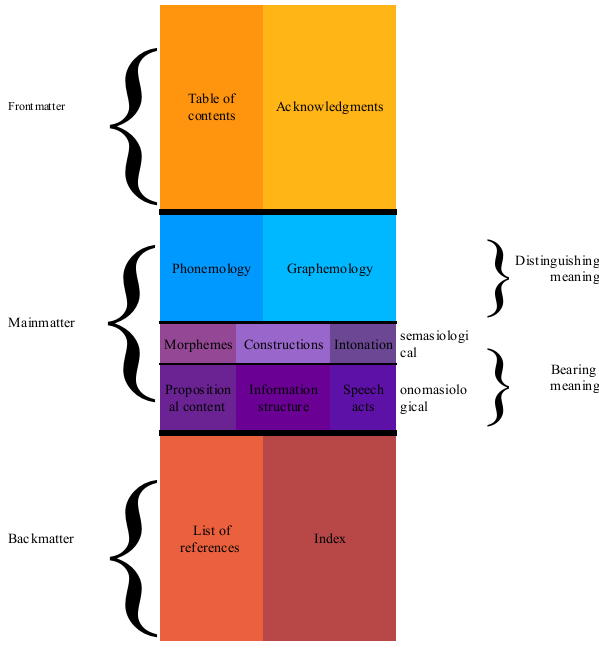
\includegraphics[width=\textwidth]{boxplot.png}
 \caption{A boxplot of the structure of grammatical descriptions}
  \label{fig:boxplot}
\end{figure}


\section{Incorporation}
A minute annotation of each document is clearly a desideratum as the above sections have shown, but it will take too much time to manually annotate even only the most significant works. Therefore, we have to use computational techniques. We use 7500 scanned and OCRed grammatical descriptions to test scalability. The first part will be to divide the works into sections. This can be done using pattern matching, and we are getting quite good results here. Related to this is the recognition of linguistic examples, which requires more sophisticated pattern matching. The ODIN project\footnote{ODIN} has achieved some success in this domain. The second step is named entity recognition. We have not started working on this yet. The third step is an automatic semantic analysis of each section. We are currently working on Latent Semantic Analysis \citep{DeerwesterEtAl1990} of the 120000 sections we extracted and will report our results in future publications.
% 
% One question which arises when conceiving such as schema is: ``Where will the content come from?'' There are two possible sources of content: Legacy descriptions, which are converted into this schema, and new descriptions, which are already written with this schema in mind.
% 
% As for legacy descriptions, we avail of several thousand pdfs, which were OCR'ed. The text was extracted and we applied some pattern matching to see whether we could partition the text into meaningful sections. We had 7845 documents in our starting set. Of those, 1436 could be split into sections. Our domain knowledge tells us that grammatical descriptions are quite granular, and that we expect a section to span between half a page and ten pages. Some of these documents have very few sections (2 or 3), suggesting a misparse. Others have thousands of sections, again suggesting a misparse. A graph showing the distribution of sections on documents is given in Figure \ref{fig:sectionsperdoc}.
% 
% \begin{figure}
% % \includegraphics[width=\textwidth]{sectionsperdoc.png}
% \caption{A plot of the number of documents which have at least the number of sections given on the X-axis}
% \end{figure}
% 
% To give some illustrative examples: 1087 documents have between 10 and 1000 sections, 808 have between 50 and 500 sections.
% 
% The next step is further annotation of the section as to their internal structure. This involves named entity recognition, and recognition of object-language words. We have not undertaken named-entity recognition yet. Object-language words cannot be found from the txt-export of an OCR-ed document, but the XML-export of Acrobat allows to find items in italics. These can then be matched with items in the textfile and marked as object language. One issue is that some object language words might also be metalanguage words and vice versa. For the time being, we use a spell checker to determine which words are not English, and are hence object language.
% 
% Recognition of examples is easy in some cases, as they have a very particular layout. They typically start with (X) where X is a number, consist of rather short lines, and the last line is enclosed in quotation marks. This heuristic has about 40\% recall. We are working on more sophisticated methods. The reader is referred to \citet{ODIN} for more information about the extraction of examples from running text.
% 
% Next to the recognition of the structure of a section, we are also interested in a description of its content. The section heading, if available, is often very informative (\em Denominal verbalization\em), but very often it is not the kind of information we require (\em Suffix -pa \em), or it is not informative (\em Other types\em).
% More information can be gathered from the body of the section. Here we use Latent Semantic Analysis \citep{abc} to group similar documents/sections together. It is hoped that at least one of those documents will have a useful semantic annotation derivable from the header which can then be cloned for the other documents in the group. One problem is that LSA works on strings and does not distinguish object language from metalanguage. For the semantic analysis, only metalanguage is interesting. If the object language is not weeded out first, all documents treating Spanish will be alike by virtue of containing \em el, la, los, las, de, y, en\em, and a document on Spanish nominalization might be found in a group with a document on Spanish prosody rather than with a document on Gujarati nominalization. By identifying object language terms in the way described above and excluding them from the LSA, this can be circumvented, but we have not gotten there yet.

So far for the legacy content. As far as future content is concerned, the application of the schema will be the easier if the authoring software is compatible with the schema on a semantic and a syntactic level. We have made good experiences with the conversion of documents written in LaTeX and HTML. The GALOES grammar authoring platform currently stores text files, but can be made to store DocBook, which will be a very good input format for a schematization process. This is on our agenda for the future.

The direct link between a semantically structured grammar authoring environment and an archive would mean that the task of the archiver changes from an iteration of acquire-conform- incorporate-acquire-conform-incorporate to a more continuous model, where granular pieces of archive material automatically find their place in the archive.

For the production of linguistic knowledge, this system means that the traditional cycle of gather-process-condense-publish-archive will be compressed, and that the primary data (gather) the transcription (process) and the analyses (condense) can be archived as they are gathered without going through the intermediate stage of a book publication. This is thus a movement towards micropublications in the sense of \citet{Cysouw2009micropub}.


\bibliographystyle{natuva}
\bibliography{nordhoff,hhling,grammaticography,asw,grammars,malay,hh,compu}

\end{document}